\documentclass{report}
\usepackage[toc,section=section]{glossaries}
\usepackage{tikz}
\usetikzlibrary{fit,arrows,automata}
\usepackage{listings, listings-rust}
\usepackage{titlesec}
\setcounter{secnumdepth}{4}

\tikzset{
    vertex/.style={
        circle,
        fill    = blue,
        outer sep = 2pt,
        inner sep = 1pt,
    }
}

%opening
\title{%
    EDB: Debugger for Ethereum's Programming Languages \\
	\medskip
	\large Report \#4: System Design \\
    \large Advised by Dr. Jackowitz	\\
	\large University of Scranton}
\author{Andrew Plaza}

\newglossaryentry{vscode}{name=Visual Studio Code, description={A popular code editor created by Microsoft}}
\newglossaryentry{rpc}{name=JSON-RPC, description={'Remote Procedure Call' is a protocol specification that outlines how a server should react to data sent to it. A JSON-RPC is an RPC that takes data in the JSON format}}
\newglossaryentry{ethereum}{name=ethereum, description={an open-source, public, blockchain-based distributed computing platform and operating system featuring smart contract functionality}}
\newglossaryentry{blockchain}{name=blockchain, description={A growing list of records stored using some datastructure (usually a variation of a tree) and linked through cryptography}}
\newglossaryentry{ethnode}{name=Ethereum Test Node, description={A Test Node which emulates the functions of a real Ethereum Node. A Test node is not connected to the rest of the Ethereum Network, and is only active on the local machine}}
\newglossaryentry{evm}{name=Ethereum Virtual Machine, description={A stack-based virtual machine with 256bit wordsize. The stack has a maximum size of 1024 elements. The memory is a word-addressed byte-array. The EVM also includes non-volatile storage which is maintained as part of the system state (state of ethereum, but not necessarily included in the blockchain). This is a word-addressed word-array. Only the hash of the storage elements is stored on the blockchain (to decrease storage costs). The EVM is used to execute bytecode formulated for it. All languages used on Ethereum compile to Ethereum Bytecode}}
\newglossaryentry{solidity}{name=Solidity, description={A Javascript-like Programming Language that compiles down to EVM Bytecode}}
\newglossaryentry{contract}{name=Smart Contract, description={'Self-Executing' code that is executed on Ethereum. Within a contract is code that contains the agreement between two parties. This is the code that EDB will be debugging}}

\makeglossaries
\begin{document}
\maketitle
\tableofcontents
\newpage

\begin{abstract}
    EDB - short for 'Ethereum Debug' exists solely to increase the ease and decrease the complexity of developing \Glspl{contract} for Ethereum. Fundamentally, \Glspl{contract} and the \Gls{evm} are simply code that is executed by a non-standard Virtual Machine (the \Gls{evm}). Vital to this process is the ability to track and decipher how exactly the code is being executed in the \Gls{evm}. There have been mistakes costing in the hundreds of millions of dollars which are results of misunderstanding this process. \footnote{Parity \$160 Million Frozen https://www.coindesk.com/startup-lost-160-million-still-wants-shake-ethereum/}\footnote{\$31 Million Stolen https://medium.freecodecamp.org/a-hacker-stole-31m-of-ether-how-it-happened-and-what-it-means-for-ethereum-9e5dc29e33ce} Current solutions for debugging \gls{contract} are not integrated into the traditional developer workflow. Many current debuggers are hardcoded for one language, and impose certain environment constraints upon the developer, such as only being available in an online web-interface. EDB aims to create a model that any language compiling to \Gls{ethereum} bytecode may fit into, as well as a model to allow extensions into different developer environments (such as Visual Studio Code).

    EDB is created using the Rust programming language. As such, this generic model which may be implemented for different \Gls{ethereum} languages is attained through implementing a few 'Traits' offered through EDB. These traits serve to abstract the compilation and language constructs of different \Gls{ethereum} languages. I present in this document a specification of how this system will operate, and what functionality will be available for developers to use.
\end{abstract}

\newpage

\section{Introduction}
    The EDB client application may be launched via the shell with the `edb' command, which launches the main program routine for the binary. Depending upon the options the user has passed EDB, the main program will first connect to the locally-run \Gls{ethnode} the user has setup, which EDB references throughout the rest of its execution. The \gls{solidity} source code file that will be debugged must also be provided by the user. From these inputs EDB creates two of it's highest-level abstractions, the File Model and the Emulator model, which make up the functionality of the debugger. The file model handles objects created by the compilation of the target source-language, such as the Abstract Syntax Tree, Source Mappings, and Bytecode. The Emulator model handles execution control and stores the \Gls{evm} (EVM) state at different steps in execution. State that is stored includes the current \Gls{evm} Stack, Memory, and Non-Volatile Storage. Internally, the Emulator model uses the `sputnikvm' library\footnote{sputnikvm https://github.com/ETCDEVTeam/sputnikvm}. These parts make up the core of the debuggers functionality. Built on top of these items is also an optional \Gls{rpc}, which may be used in order to build featureful Graphical User Interfaces from 3rd-party applications.

    The design of EDB started first with a general development plan where models that were needed were identified. Based upon this plan, generic interfaces were created based upon the needs of the structure. Once this was complete, development was constrained to one part or sub-part of one model/interface, which worked towards fitting into the generic interface that was created during the first step. Unit tests were created alongside the original development of the part or sub-part, and testing took place to ensure the part worked individually before moving on to connect the part with the rest of the program. A kanban board on `Github Projects` was used in order to keep track of work that is under development, finished, or needs to be started.

\section{Levels}
\subsection{High Level System Model}

\begin{figure}[!h]
    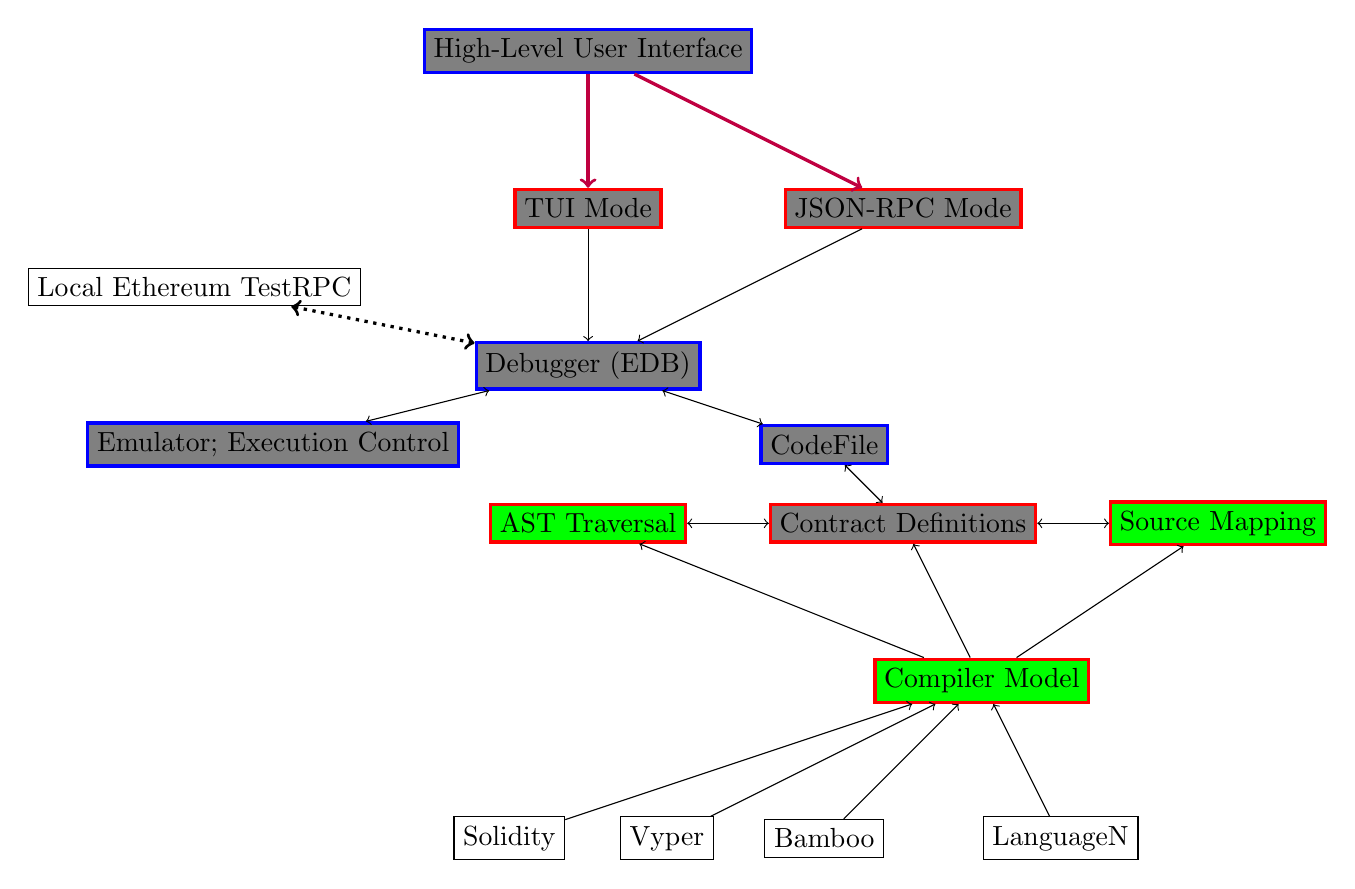
\begin{tikzpicture}

		\node[draw=blue,fill=gray,very thick] (CLI) at (8,10) {High-Level User Interface};

		\node[draw=red,fill=gray,very thick] (JSONRPC) at (12, 8) {JSON-RPC Mode};
		\node[draw=red,fill=gray,very thick] (TUIMode) at (8, 8) {TUI Mode};

		\node[draw] (ETH) at (3,7) {Local Ethereum TestRPC};

        \node[draw=blue,fill=gray,very thick] (EDB) at (8,6) {Debugger (EDB)};
        \node[draw=blue,fill=gray,very thick] (EVM) at (4, 5) {Emulator; Execution Control};
        \node[draw=blue,fill=gray,very thick] (CodeFile) at (11,5) {CodeFile};

        \node[draw=red,fill=green,very thick] (AST) at (8, 4) {AST Traversal};
        \node[draw=red,fill=gray,very thick] (Contracts) at (12, 4) {Contract Definitions};
        \node[draw=red,fill=green,very thick] (SrcMaps) at (16, 4) {Source Mapping};

        \node[draw=red,fill=green,very thick] (Compiler) at (13, 2) {Compiler Model};
        \node[draw] (Solidity) at (7, 0) {Solidity};
        \node[draw] (Vyper) at (9, 0) {Vyper};
        \node[draw] (Bamboo) at (11, 0) {Bamboo};
        \node[draw] (LanguageN) at (14,0) {LanguageN};

		\draw[->,draw=purple,very thick] (CLI) to (JSONRPC);
		\draw[->,draw=purple,very thick] (CLI) to (TUIMode);

		\draw[->,draw=black] (JSONRPC) to (EDB);
		\draw[->,draw=black] (TUIMode) to (EDB);


        \draw[<->,draw=black] (EDB) to (EVM);
        \draw[<->,draw=black] (EDB) to (CodeFile);
		\draw[<->,draw=black,dotted,very thick] (EDB) to (ETH);

        \draw[<->,draw=black] (Contracts) to (AST);
        \draw[<->,draw=black] (Contracts) to (SrcMaps);
        \draw[<->,draw=black] (CodeFile) to (Contracts);

        \draw[<-,draw=black] (AST) to (Compiler);
        \draw[<-,draw=black] (SrcMaps) to (Compiler);
        \draw[<-,draw=black] (Contracts) to (Compiler);

        \draw[->,draw=black] (Solidity) to (Compiler);
        \draw[->,draw=black] (Vyper) to (Compiler);
        \draw[->,draw=black] (Bamboo) to (Compiler);
        \draw[->,draw=black] (LanguageN) to (Compiler);
        %%% Color Legend
	\end{tikzpicture}
    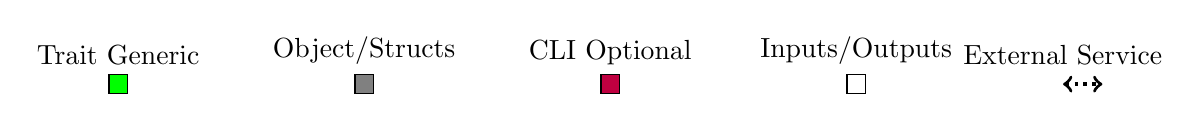
\begin{tikzpicture}
        \node [label=Trait Generic,draw,fill=green] (node1) {};
        \node [label={[name=l] Object/Structs},draw,fill=gray] (node2) at ([xshift=3cm]node1.east){};
        \node [label={[name=l] CLI Optional},draw,fill=purple] (node3) at ([xshift=3cm]node2.east){};
        \node [label={[name=l] Inputs/Outputs},draw] (node4) at ([xshift=3cm]node3.east){};
        \node [label={[name=l] External Service}] (node5) at ([xshift=2.5cm]node4.east){};
        \draw [<->,draw=black,dotted,very thick] (12,0) to (12.5,0);
    \end{tikzpicture}
    \vspace*{1cm}

    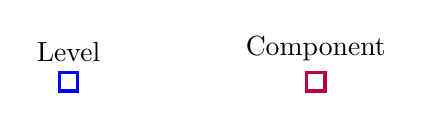
\begin{tikzpicture}
        \node [label=Level,draw=blue,very thick] (node1) {};
        \node [label={[name=l] Component},draw=purple, very thick] (node2) at ([xshift=3cm]node1.east){};
    \end{tikzpicture}
    \caption{High Level System Model}
\end{figure}
\newpage

\subsection{High Level User Interface}
\subsubsection{Abstract Specification}
    When a user downloads and installs EDB onto their machine of choice, it comes as a CLI app, `edb` that may be launched from the command line. There are two modes EDB may be used in, `Text User Interface (TUI) mode` as a standalone debugger, or '\Gls{rpc}' mode, in case a developer wants to build a featureful GUI using EDB. A developer may access this GUI by forking the `edb` application from within their program. In order to debug a program, some arguments, not dependent on the 'mode' edb is being launched in, are required. These arguments are the path to the source code file, and the name of the contract that is being debugged. The High-Level UI contains two general components: TUI Mode and \Gls{rpc} mode. These two 'modes' are targeted at different users. The TUI mode is a standalone-debugger for users who wish to use the most basic form of EDB as a Command-Line interface. The \Gls{rpc} mode is targeted at developers who wish to extend the features of EDB into a third-party and full-featured Graphical User Interface. An example could be a \Gls{vscode} plugin which forks the `edb' program in \Gls{rpc} mode, in order to integrate the features of EDB with \Gls{vscode}.

\subsubsection{Interface Design}
    The high level user interface only exposes functionality in the form of a compiled command-line application, and not as a library. No other subparts from the EDB structure will interface with the command-line application. The UI, however, will interface with the 'CodeFile' and 'Emulator' libraries in order to provide debugging functionality. The \Gls{rpc}, however, exposes functions that are necessary for featureful third-party applications that may wish to use EDB's functionality in their own program. In this case, the \Gls{rpc} must provide functions for loading source code, stepping through source code, setting breakpoints, and exposing EVM state in the form of human-readable variables, storage, and stack elements.

\subsubsection{Component: TUI Mode}
    The default mode for launching EDB is TUI mode. Therefore, no extra arguments to `edb` are required to launch the TUI environment. TUI mode is launched through the native command-prompt of the operating system. This may be a Terminal Emulator and Shell of choice on UNIX environments, or Powershell/CMD on Windows. Once a user launches EDB with the required options (source code file and the name of the contract), the debugger's TUI mode takes over the terminal, and a prompt where the user may specify commands to provide to edb is made available. Examples of commands the user may input are 'step', 'break', 'next', and 'restart'. However, the debugger TUI will provide as many commands as necessary to make debugging of \gls{contract} possible. This includes stepping forward and backward in code, seeing the current stack, setting and removing breakpoints, as well as viewing local/global variables and their values.

\subsubsection{Component: JSON-RPC Mode}
    The \Gls{rpc} mode provides full-featured functionality of EDB much like the TUI mode does. The difference, however, is just how a user may interact with the interface. \Gls{rpc} mode launches EDB and expects the debugger to be used in a client-server model. This is to facilitate integration into third-party applications, while allowing third-party implementations to remain independant of EDB.

    \begin{figure}[h]
        \centering
        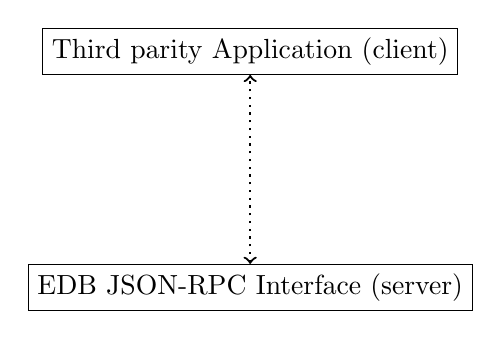
\begin{tikzpicture}
            \node[draw] (EDB) at (0,0) { EDB JSON-RPC Interface (server)};
            \node[draw] (Third-Party) at (0, 3) {Third parity Application (client)};
            \draw[<->,draw,dotted,thick] (EDB) to (Third-Party);
        \end{tikzpicture}
        \caption{EDB Client-Server}
    \end{figure}

\subsection{Debugger Core, EDB}
    \subsubsection{Abstract Specification}
        The Debugger core provides all the core debugging features one may expect a debugger to offer. This level is not concerned with parsing input or events that the user may trigger. Instead, it works with input that has already been parsed. Namely, the \Gls{ethereum} Language Trait, a \Gls{rpc} Client, and parameters for the transaction the user wishes to debug. Sourcemapping and EVM Execution control is done implicitly through the debug functions: 'step', 'next', 'stop', 'restart', etc. Therefore, this level mostly serves as a higher-level abstraction over the next two levels 'Emulator' and 'CodeFile'. This level accepts the source code file, a object which implements the trait 'Language', a \Gls{rpc} client to communicate with the locally running \Gls{ethnode}, along with the block and transaction the user wishes to debug. From these inputs, creation of the Emulation and Source Mapping objects is enabled.
    \begin{figure}
        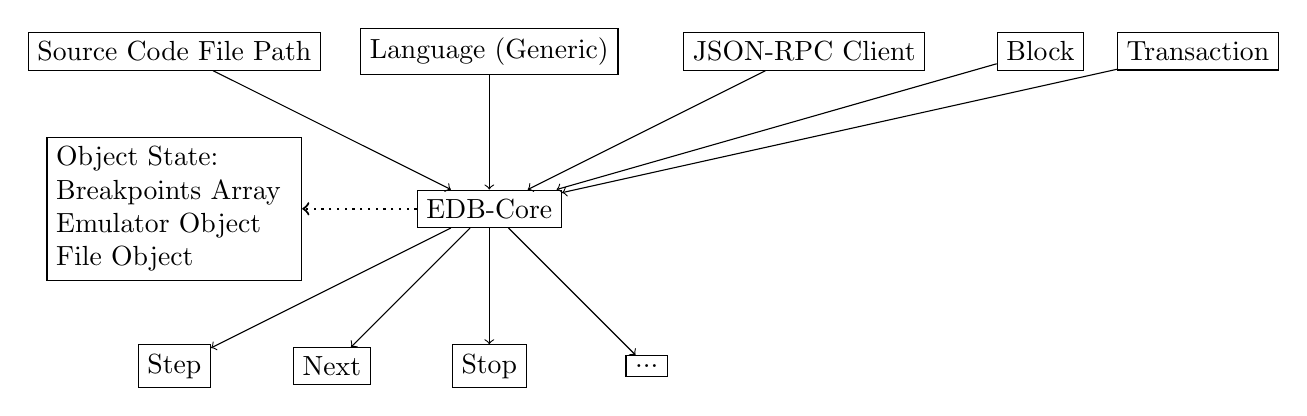
\begin{tikzpicture}
            \node[draw] (File) at (0,4) {Source Code File Path};
            \node[draw] (Language) at (4,4) {Language (Generic)};
            \node[draw] (Client) at (8,4) {JSON-RPC Client};
            \node[draw] (Block) at (11,4) {Block};
            \node[draw] (Transaction) at (13,4) {Transaction};


            \node[draw] (EDB-Core) at (4,2) {EDB-Core};

            \node[draw,text width=3cm] (Object State) at (0, 2) {Object State:\
                Breakpoints Array\
                Emulator Object\
                File Object};

            \node[draw] (Step) at (0,0) {Step};
            \node[draw] (Next) at (2,0) {Next};
            \node[draw] (Stop) at (4,0) {Stop};
            \node[draw] (etc) at (6,0) { ... };

            \draw[->,draw,dotted,thick] (EDB-Core) to (Object State);
            \draw[->,draw] (Language) to (EDB-Core);
            \draw[->,draw] (Client) to (EDB-Core);
            \draw[->,draw] (Block) to (EDB-Core);
            \draw[->,draw] (Transaction) to (EDB-Core);
            \draw[->,draw] (EDB-Core) to (Step);
            \draw[->,draw] (EDB-Core) to (Next);
            \draw[->,draw] (EDB-Core) to (Stop);
            \draw[->,draw] (EDB-Core) to (etc);
            \draw[->,draw] (File) to (EDB-Core);
        \end{tikzpicture}
        \caption{EDB Core Abstract Structure}
    \end{figure}
    \newpage

    \subsubsection{Interface Design}
        This level should be able to provide all the debug functions needed in order to debug a source code file. It should not expose any objects or functions which deal with Source Mapping or \Gls{evm} emulation. It is assumed that inputs provided to this interface match up with information that is present in the local \Gls{ethnode}. Necessarily this indicates that the compiled bytecode of the source code provided matches with bytecode that has already been deployed onto the \Gls{ethnode}. This level should provide a programmatic view of the functions outlined in the requirements specification, namely:
    \begin{itemize}
        \item \textbf{step}: step forward to the next source-line in execution
        \item \textbf{stepback}: step back one source-line in execution
        \item \textbf{print}: print stack, memory, or variables in the program
        \item \textbf{printline}: print the current line in the source code that execution is at
        % \item \textbf{printlines}: print a number of lines relative to the current line code execution is at in source code
        %\item \textbf{set_breakpoint}: set a breakpoint at a line number in the source code where execution will stop
        %\item \textbf{unset_breakpoint}: Unset a breakpoint at a line number
        \item \textbf{restart}: restart execution entirely from a clean Ethereum Virtual Machine state
        \item \textbf{run}: run a function in the source code (accepts arguments according to function parameters)
        \item \textbf{next}: Continue execution to the next breakpoint
        \item \textbf{previous}: Take execution back to the previous breakpoint
        \item \textbf{stepinto}: Step into a function (if the current line contains a function call)
    \end{itemize}

    \subsubsection{Component: Address Cache}
        In order to associate information provided by the user in the form of a source code file, a component to match up the compiled bytecode created from the file provided by the user to an address existing in the \Gls{ethnode} is necessary. This information is needed throughout transaction execution in case the \Gls{evm} is in need of any state existing on the blockchain before execution has started. Therefore, a local cache of all known addresses and associated compiled bytecode is created once the debugger is first launched. This cache is stored as a HashMap: The key is a 160bit address (The Address of the Ethereum Account owning the code) and the value is the compiled bytecode. This information is gathered and updated whenever the EDB client is run by crawling all addresses known to the \Gls{ethnode}. It is up to the user whether to refresh this information on each run of the debugger. If a refresh is desired, no data related to addresses needs to be stored on-disk.  Otherwise, data crawled from the \Gls{ethnode} is stored on-disk to be optionally loaded on the next run of the debugger. Since only one contract is being debugged at a time, the address cache is only queried once for the relevant address and bytecode. The cache object is not stored along with the Object State, since later retrieval may be done via the filesystem if requested by the user.
    \begin{figure}[!h]
        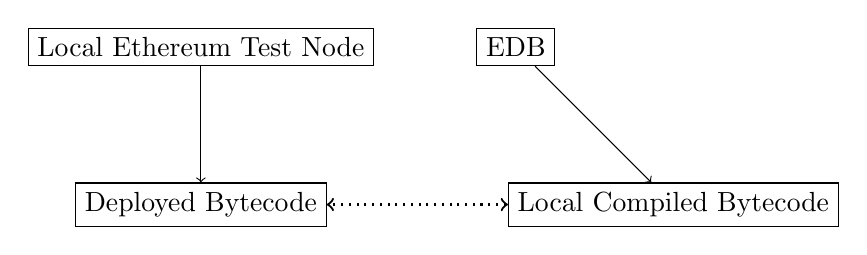
\begin{tikzpicture}
            \node[draw] (TestNode) at (0, 4) {Local Ethereum Test Node};
            \node[draw] (DeployedBytecode) at (0, 2) {Deployed Bytecode};
            \node[draw] (EDB) at (4, 4) {EDB};
            \node[draw] (LocalBytecode) at (6, 2) { Local Compiled Bytecode};

            \draw[->,draw] (TestNode) to (DeployedBytecode);
            \draw[->,draw] (EDB) to (LocalBytecode);
            \draw[<->,draw,dotted,thick] (LocalBytecode) to (DeployedBytecode);
        \end{tikzpicture}
        \caption{Address mapping from Local Node to EDB Application}
    \end{figure}

    \subsubsection{Component: Breakpoints}
        Breakpoints are set and unset by two functions 'set\_breakpoint' and 'unset\_breakpoint'. These are stored in a simple array. Each breakpoint serves as an indicator as to where execution should stop for the rest of the debug functions. For instance, in order to begin debugging the `set\_breakpoint' function of the EDB interface is called first. Once `run' is called after that, execution is expected to continue up to and only until that line in the original source code file. Each consequent `step' call is expected to run only until the next line in the source code, while a `next' call would be expected to run to the next breakpoint.

\subsection{Emulator, Execution Control}

    \subsubsection{Abstract Specification}
        The Emulator provides execution control for the debugger level. This means it deals at the Opcode and Instruction level, stores and exposes state related to the Ethereum Virtual Machine, and handles any blockchain state requirements it may need from the \Gls{ethnode}. The 'Transaction' and 'Block' inputs mostly contain extraneous information that is unnecessary to debugging but necessary to general Ethereum Transaction Execution, except for the bytecode which is apart of the 'Transaction' input object. The Emulator, however, is not concerned with lines in the source code, breakpoints, or any 'human-decipherable' meaning which may be attached to items that reside in the Ethereum Virtual Machine state. It is able to decipher individual opcodes from Instructions, as well as identify how those opcodes contribute to the next state of the Ethereum Virtual Machine. At it's lowest level, an Ethereum Virtual Machine library, `sputnikvm` is used in order to carry out these instructions and general code execution. In addition, the Emulator keeps the Stack, Memory, and Non-Volatile storage in sync with the \Gls{ethnode}, and is able to access these data-structures at-will (without any constraints).
    \begin{figure}[!h]
        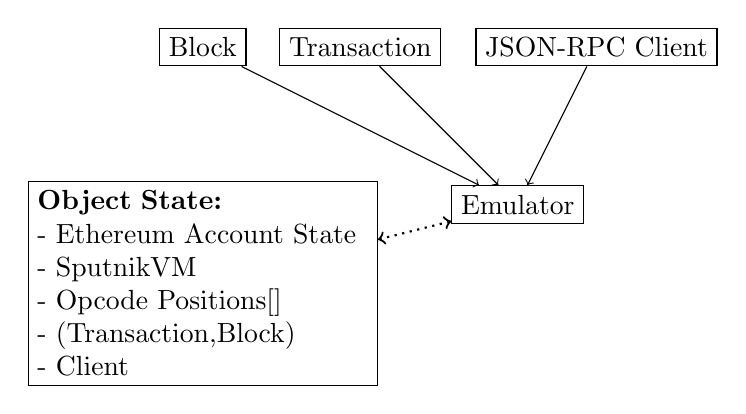
\begin{tikzpicture}
            \node[draw] (Block) at (0, 4) {Block};
            \node[draw] (Transaction) at (2, 4) {Transaction};
            \node[draw] (Client) at (5,4) {JSON-RPC Client};
             \node[draw] (Emulator) at (4, 2) { Emulator };

            \node[draw,text width=4.2cm] (Object State) at (0, 1) {\textbf{Object State:}\\
                    - Ethereum Account State\\
                    - SputnikVM\\
                    - Opcode Positions[]\\
                    - (Transaction,Block)\\
                    - Client\\};
            \draw[->,draw] (Block) to (Emulator);
            \draw[->,draw] (Transaction) to (Emulator);
            \draw[->,draw] (Client) to (Emulator);
            \draw[<->,draw,dotted,thick] (Emulator) to (Object State);

        \end{tikzpicture}
        \caption{Emulator Abstract Structure}
    \end{figure}

    \subsubsection{Interface Design}
        The interface of the Debugger and Emulator level hold many similiarites. For instance, the Emulator is able to `step\_forward`, `step\_back`, and `run\_until` a certain point in execution has been reached. However, instead of stepping over lines in source code, functions at the Emulator level deal only with stepping instructions in the bytecode. Therefore, 'step\_forward' means execute the next instruction in the bytecode array, and 'step\_back' means to step back to the overall state before the current instruction had been executed. Functions to peek at the current state of the Virtual Machine are also exposed, in order to faciliate variable-decoding at in the Debugger level.

    \subsubsection{Algorithm Design}

\begin{figure}[h]
\centering
    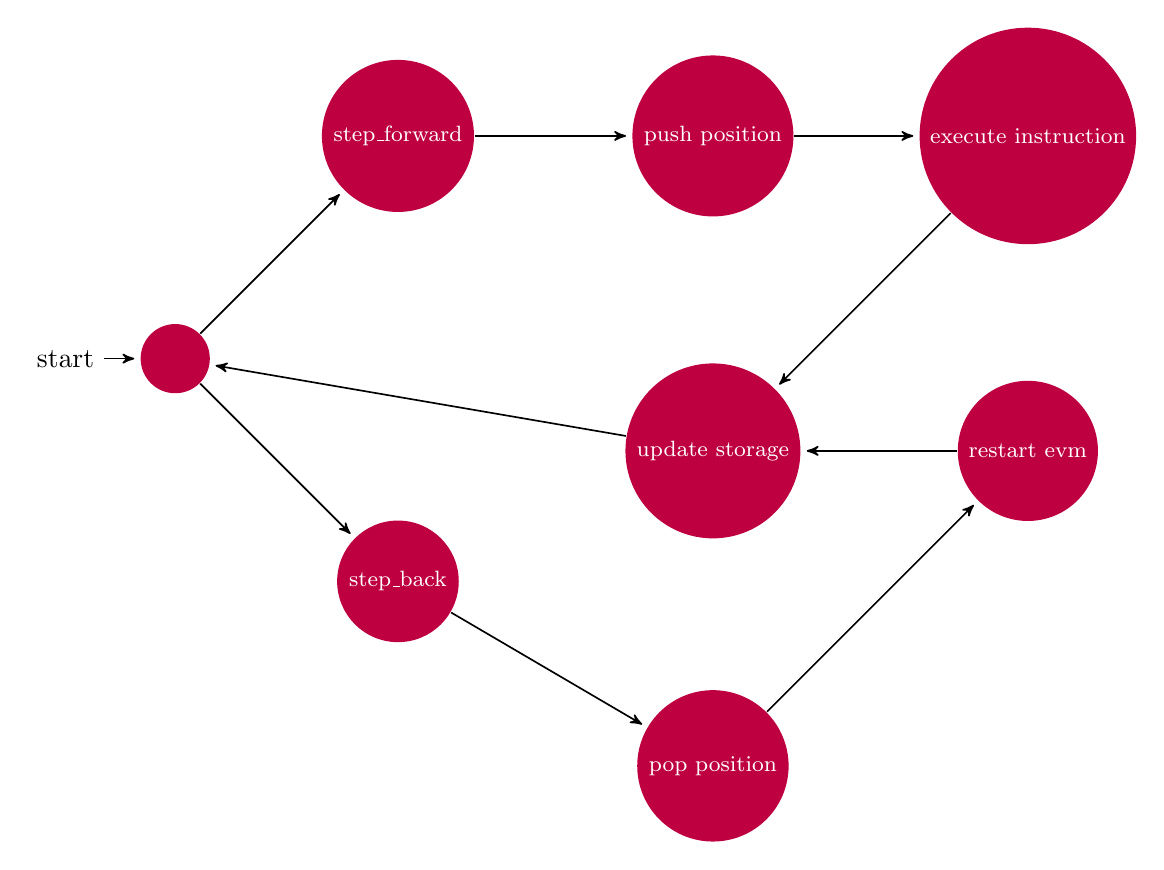
\begin{tikzpicture}[->,>=stealth',shorten >=2pt,auto,node distance=4cm,semithick]
        \tikzstyle{every state}=[fill=purple,draw=none,text=white]

        \node[initial,state] (A)                    {};
        \node[state]         (B) [above right of=A] {\footnotesize step\_forward};
        \node[state]         (D) [below right of=A] {\footnotesize step\_back};
        \node[state]         (C) [right of=B]       {\footnotesize push position};
		\node[state]	     (H) [right of=C]		{\footnotesize execute instruction};
        \node[state]         (E) [below of=C]       {\footnotesize update storage};
        \node[state]         (F) [below of=E]       {\footnotesize pop position};
        \node[state]         (G) [right of=E]       {\footnotesize restart evm};

    \path   (A) edge              node {} (B)
                edge              node {} (D)
            (B) edge              node {} (C)
            (C) edge              node {} (H)
            (D) edge              node {} (F)
            (E) edge              node {}       (A)
            (F) edge              node {} (G)
            (G) edge              node {} (E)
			(H) edge			  node {} (E);
                %edge              node {0,1,R} (A);
            % (E) edge [bend left]  node {1,0,R} (A);
    \end{tikzpicture}
    \caption{Algorithmic Design of Execution Control}
\end{figure}

        There are two main parts of the Emulators Algorithm Design: In-Memory representation of Non-Volatile Storage, and states of the EVM.
        \newpage

    \vspace{0.5cm}

    \textbf{Emulator States}:

    \vspace{0.5cm}

        The Emulator is required to have the ability to reference all state of the Ethereum Virtual Machine of executing code during any point in execution. This means that the Stack and Memory for every line in source code must be stored or referenced in some capacity. This is done in order to facilitate stepping through all possible points in execution (including stepping backward). The easiest way of doing so would be to save a copy of the EVM Stack, Memory, and Program Counter as a tuple in a dynamically-sized stack. The top of the stack would be the previous state of the Ethereum Virtual Machine. If a user needs to step back, then this state-stack could be popped and the resulting states in the EVM reverted. This, however, may require a large amount of memory depending on the size of the program, and would increase considerably if the Ethereum Smart Contract were to call an external library. This is because an external library requires its own and entirely seperate EVM Stack, Memory (CITE ETHEREUM YELLOW PAPER) (As per the specification in the Ethereum Yellow Paper). The actual execution of smart contracts, however, is relatively inexpensive. Therefore, in order to decrease the memory-footprint of the Emulator, only the opcode-position in the bytecode-array of the corresponding line in source code is stored by the Emulator in a dynamically-sized stack. If a user wishes to step back, the current EVM state is first totally wiped, the positions-vector popped, and the EVM re-run to the corresponding opcode position that was popped from the positions vector therefore re-populating the EVM Stack and Memory to its previous state.

        \vspace{0.5cm}

        \textbf{Non-Volatile Storage}

        \vspace{0.5cm}

            A user may want to chain a second (or more) transactions after executing one transaction that acts on the state from the first transaction. Therefore, the state of non-volatile storage is kept track of on a per-contract basis that is seperate from the state stored in the \Gls{ethnode}. If the user needs to step back, the state changed only from the currently-executing contract is wiped and re-populated along with the EVM state. This state is kept in a nested hashmap, where the first level of the hashmap is a mapping between account addresses (160bit hashes) and a hashmap. The second level is a mapping between unsigned-256bit integers and unsigned-256bit integer. This second level is the 'Non-Volatile' storage for a particular smart contract identified by an account address at the first level.

    \subsubsection{Component: Persistant Account State}
        In order to facilitate a clean test environment for users wishing to test code, there must be an aspect of seperation from the verbatim \Gls{ethnode} State. In other words, the debugger must present an environment where the user may manipulate and mutate their program without having to worry about affecting any change in the node that is running locally, and before committing the changes to the node. This is done sequentially:
        \begin{enumerate}
            \item Pull the current state from the local \Gls{ethnode} before execution of the user's program
            \item Handle state updates originating from users program that is being debugged within the debugger
            \item Allow user to run other functions/programs/mutate the state further based based on the previously debugged program (chaining execution)
            \item Provide an option to commit all state changes to \Gls{ethnode} if debugging is finished
        \end{enumerate}

    \subsubsection{Component: Opcode and Instruction Mappings}
        A requirement of the emulator is to handle the current position in the bytecode that is being executed. This includes deciphering the current instruction being executed. Fortunately, the \Gls{ethereum} virtual machine is a stack-based architecture, so the only instruction with operands is the `\textbf{PUSH}` instructions (PUSH1-PUSH32). The currently-executing opcode position is kept track of in the EVM. So, in order to find the current instruction being executed, the bytecode array is walked. If this iteration comes across a PUSH instruction, the operands succeeding the opcode are skipped (the instruciton counter not incremented). Therefore, the emulator has a way to return the index of the current instruction being executed. This is required for Source Mapping (in later levels).

\subsection{CodeFile}
    \subsubsection{Abstract Specification}
        The CodeFile must provide all functions which allow the deciphering and manipulation of Source Code, Bytecode, and the AST. The CodeFile Object itself is an abstraction on top  of a number of different components. Some of these components are made generic in order to facilitate a model which may be implemented for any arbitrary \Gls{ethereum} Language which compiles to \Gls{ethereum} bytecode. Parts of \Gls{ethereum} Languages are constant across all languages, such as Contract ABI. These parts, therefore, do not need to be made generic and are implemented as simple struct objects. The CodeFile does not have access to any execution environment such as the \gls{evm}.
    \newpage
    \begin{figure}[!h]
        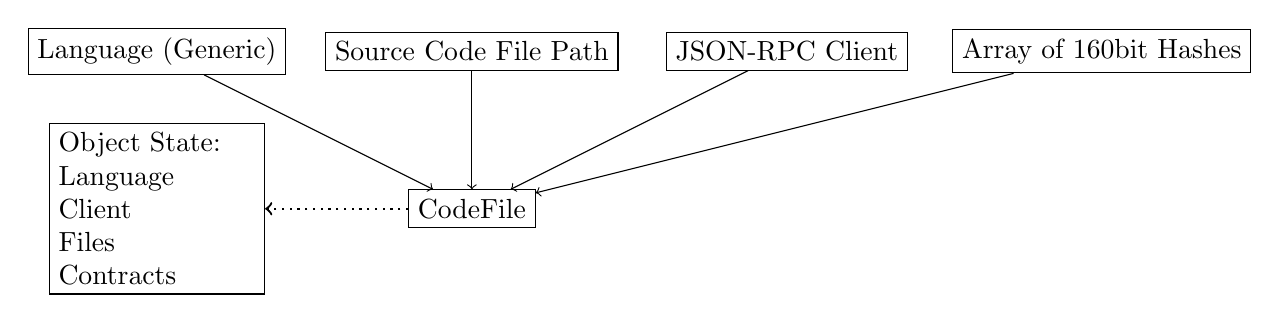
\begin{tikzpicture}
            \node[draw] (Language) at (0,4) {Language (Generic)};
            \node[draw] (File) at (4,4) {Source Code File Path};
            \node[draw] (Client) at (8,4) {JSON-RPC Client};
            \node[draw] (Addresses) at (12,4) {Array of 160bit Hashes};
            \node[draw] (CodeFile) at (4,2) {CodeFile};

            \node[draw,text width=2.5cm] (Object State) at (0, 2) {Object State:\\
                Language\\
                Client\\
                Files\\
                Contracts
            };

            \draw[->,draw,dotted, thick] (CodeFile) to (Object State);
            \draw[->,draw] (File) to (CodeFile);
            \draw[->,draw] (Language) to (CodeFile);
            \draw[->,draw] (Client) to (CodeFile);
            \draw[->,draw] (Addresses) to (CodeFile);
        \end{tikzpicture}
        \caption{CodeFile Abstract Structure}
    \end{figure}

    \subsubsection{Interface Design}
		First, this level needs to manage source code files and any external libraries they may reference. This constitutes compiling the source code file specified by the user, and then compiling any library which may be included inside of the original source code file. This level must provide the ability to map arbitrary positions in bytecode (based on the instruction offset) to lines in source code files. Additionally, it must provide a general contract interface derived from Contract ABI's to faciliate decoding function parameters, and calling contract functions. Lastly, an interface for finding the positions of functions in the source code, and the positions of variable declarations needs to exist.

    \subsubsection{Component: Contract File}
    \begin{figure}
        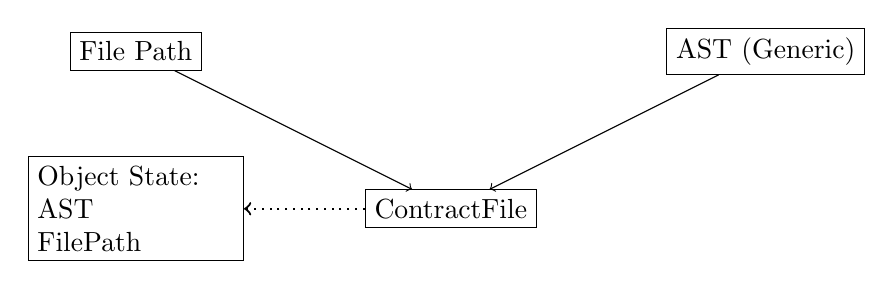
\begin{tikzpicture}
            \node[draw] (File Path) at (0,4) {File Path};
            \node[draw] (AST) at (8,4) {AST (Generic)};

            \node[draw] (ContractFile) at (4,2) {ContractFile};

            \node[draw,text width=2.5cm] (Object State) at (0, 2) {Object State:\\
                AST\\
                FilePath\\
            };

            \draw[->,draw,dotted, thick] (ContractFile) to (Object State);
            \draw[->,draw] (AST) to (ContractFile);
            \draw[->,draw] (File Path) to (ContractFile);
        \end{tikzpicture}
        \caption{Contract File Abstract Structure}
    \end{figure}

	The ContractFile corresponds 1:1 with a file that is on the users filesystem. The AST of the sourcefile is stored within this Contract File Object, since the AST encompasses the entire file and not just one class or section in the Source Code. Therefore, it is mainly through this structure that higher levels may access the Generic AST Traversel methods.

	\newpage
    \subsubsection{Component: Contract}
        A Contract is an abstraction over the \Gls{contract} ABI (CITE SPEC), and the Source Map generated by the compiler. Every contract references the ContractFile Object it originated from. `Contract` provides functions which allow for calling methods on the contract which exist on the \Gls{ethnode}. In addition, this ABI specifies all functions, their parameters and types in one Contract definition. This is where the bytecode that was compiled is matched with the bytecode that exists on the Local \Gls{ethnode}. Additionally, the Generic Source Map trait and it's associated functions may also be accessed.
    \begin{figure}[!h]
        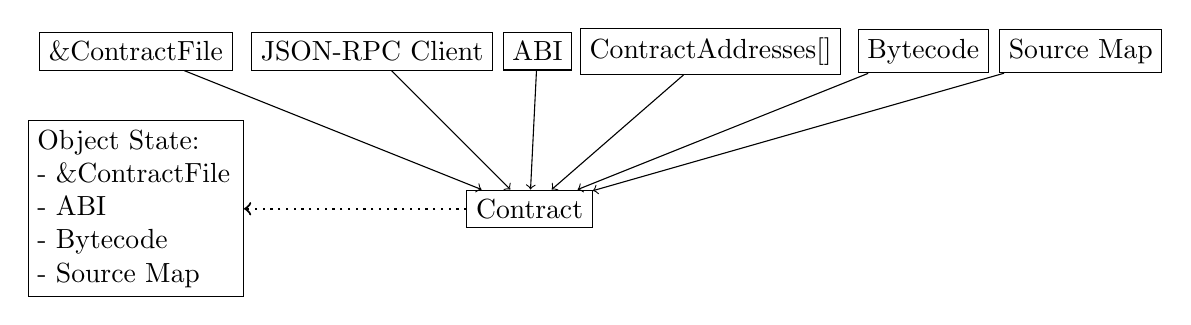
\begin{tikzpicture}
            \node[draw] (File) at (0,4) {\&ContractFile};
            \node[draw] (Client) at (3,4) {JSON-RPC Client};
            \node[draw] (ABI) at (5.1,4) { ABI};
            \node[draw] (Addresses) at (7.3, 4) {ContractAddresses[]};
            \node[draw] (Bytecode) at (10,4) {Bytecode};
            \node[draw] (Source Map) at (12, 4) {Source Map};

            \node[draw] (Contract) at (5,2) {Contract};
            \node[draw,text width=2.5cm] (Object State) at (0, 2) {Object State:\\
                - \&ContractFile\\
                - ABI\\
                - Bytecode\\
                - Source Map\\
            };

            \draw[->,draw,dotted, thick] (Contract) to (Object State);
            \draw[->,draw] (File) to (Contract);
            \draw[->,draw] (Client) to (Contract);
            \draw[->,draw] (ABI) to (Contract);
            \draw[->,draw] (Addresses) to (Contract);
            \draw[->,draw] (Bytecode) to (Contract);
            \draw[->,draw] (Source Map) to (Contract);
        \end{tikzpicture}
        \caption{Contract Abstract Structure}
    \end{figure}

	\subsubsection{Component: AST Traversal}
		AST Traversel is a Generic Trait which specifies how a language must be implemented in order to fit into EDB's model for debugging. Variables, Functions, and Contract definitions are abstracted to only include information that is needed for debugging. This, however, serves two purposes:
	\begin{enumerate}
		\item Since every language is free to implement the Abstract Syntax Tree and its types however it needs, then there can be no clear structures to store this data. Therefore an abstract model is created to specify how the data should be stored
		\item Raw AST nodes need not be accessed, since most of the information will be unused. Therefore, the AST trait only includes functions that would be useful for debugging purposes (such as finding function definitions and their location in the source code, or finding variable declarations and their position in source code.)
	\end{enumerate}
	For some purposes, however, more specific details may be needed on a case-by-case or language-by-language basis. In order to faciliate this, the `AbstractFunction` Trait Generic allows for more fine-grained control of iterating through the AST Nodes specific to functions. In this trait, the term 'function' is used loosely. For a language that does not inlude the concept of traditional 'functions' (ex: Assembly) then the parts of a subroutine may be made to fit into this model as well.

\begin{figure}[!h]
    \begin{lstlisting}[language=Rust,basicstyle=\footnotesize]
pub trait Ast {
  /// get a variable declaration
  fn variable(&self, name: &str) -> Result<AstItem, Error>;

  /// Get a contract declaration
  fn contract(&self, name: &str) -> Result<AstItem, Error>;

  /// Access a Function via a Closure
  fn function(&self, name: &str, fun: &mut FnMut(Result<&AbstractFunction, Error>) -> bool)
    -> Result<AstItem, Error>;

  /// Find a contract by it's byte offset in the source file
  fn find_contract(&self, offset: CharOffset) -> Option<AstItem>;

  /// Find a function via the closure `fun`. The abstract function from AST is passed into
  /// the closure and individual AST nodes may be accessed through it. Returns an AST item
  /// based on result of closure
  fn find_function(&self, fun: &mut FnMut(&AbstractFunction) -> bool) -> Option<AstItem>;

  /// Find variable declarations within a contract
  fn find_variables(&self, contract: &str) -> Option<Vec<AstItem>>;
}
    \end{lstlisting}
    \caption{AST Trait Specification}
\end{figure}

\begin{figure}[!h]
    \begin{lstlisting}[language=Rust,basicstyle=\footnotesize]
pub trait AbstractFunction {
  /// Name of the function
  fn name(&self) -> String;
  /// Parameters of function
  fn params(&self) -> ethabi::Param;
  /// Function Returns
  fn returns(&self) -> ethabi::Param;
  /// Any mutations to state that occur within the function
  fn mutations(&self) -> Box<Iterator<Item=Mutation>>;
  /// Source location of current AST Node
  fn location(&self) -> SourceRange;
}
    \end{lstlisting}
    \caption{Abstract Function Trait Specification}
\end{figure}

\newpage
	\subsubsection{Component: Source Mapping}
		The Source Mapping Generic Trait provides a model for source maps generated by language compilers. The requirements of a Source Map are to map Instruction offsets in the bytecode to line numbers in source code. This concept is universal to all Ethereum Languages. The format, style, and types of the source map generated by Ethereum Language Compilers, however, is not standard.

\begin{figure}[!h]
    \begin{lstlisting}[language=Rust,basicstyle=\footnotesize]
/// Represents a Source Map
pub trait SourceMap {
  /// Check if a unique instruction mapping exists
  /// Generally used for setting breakpoints
  fn unique_exists(&self, lineno: LineNo) -> bool;
  /// Get a unique linenumber mapped to an instruction position
  /// This is usually the instruction in the sourcemap with the shortest length,
  /// that matches the linenumber provided. Usually used for run_until().
  /// Generally this ignores function declarations, while() loops, and if() statements
  /// used for breakpoint handling (setting breakpoints)
  fn unique_ins_pos(&self, lineno: LineNo) -> Result<OpcodeOffset, Error>;
  /// Get the instruction offset from a line number in the Source Code.
  /// This is the first occurrence of an instruction relative to
  /// `from` offset that matches the linenumber provided. Usually used for step()
  fn ins_pos_from_lineno(&self, lineno: LineNo, from: OpcodeOffset)
	-> Result<OpcodeOffset, Error>;
  /// Get the character position in a file from a line number (Ignores leading whitespace)
  fn char_pos_from_lineno(&self, lineno: LineNo) -> Result<CharOffset, Error>;
  /// Get the LineNumber that corresponds with a character offset
  fn lineno_from_char_pos(&self, offset: CharOffset) -> Result<LineNo, Error>;
  /// Get the linenumber that corresponds to an instruction position
  fn lineno_from_ins_pos(&self, offset: OpcodeOffset) -> Result<LineNo, Error>;
  /// Get a line mapping (line number => str) from instruction position/offset
  fn current_line(&self, offset: OpcodeOffset) -> Result<Line, Error>;
  /// Get the last `count` number of lines (inclusive) from instruction position/offset
  fn last_lines(&self, offset: OpcodeOffset, count: usize) -> Result<Vec<Line>, Error>;
  /// Get the next `count` number of lines (inclusive) from instruction position/offset
  fn next_lines(&self, offset: OpcodeOffset, count: usize) -> Result<Vec<Line>, Error>;
}
    \end{lstlisting}
    \caption{Source Map Trait Specification}
\end{figure}

	\newpage
    \subsubsection{Component: Compiler}
		The 'Compiler' Generic Trait provides a model for Ethereum Languages to specify how their language should be compiled into the generics and structs needed. It is required to return a Tuple of two vectors, 'ContractFile' and 'Contract' which include the AST and SourceMap implementations respectively.
\begin{figure}[!h]
    \begin{lstlisting}[language=Rust,basicstyle=\footnotesize]
/// The Source File of a specific language
pub trait Language {

	/// Compiles Source Code File into a tuple of Vectors of (ContractFile, Contract)
	/// where every Contract holds an immutable reference back to the
	/// file it originates in
	/// (since multiple contracts may be housed in one file)
	fn compile<T>(&self,
		path: PathBuf,
		client: &web3::api::Eth<T>,
		addresses: &[Address])
	-> Result<(Vec<Rc<ContractFile>>, Vec<Contract<T>>), Error> where T: Transport;
}
    \end{lstlisting}
    \caption{Compiler Trait Specification}
\end{figure}

\section{User Interface}
    The main goal of the user interface inside the Text-User-Interface is to be as clear, concise, and simple to use as possible. The flow of the UI should be consistant and logical. The help system must be easily available, with a clear message at the launch of the application as to how to access the 'help' dialogue. The interface should remain simple, and should feel like an extension of the Shell UI rather than a totally separate application. Outside of the TUI, a manual page (for UNIX systems) will be written in order to provide context, specifics, and information on how to use EDB. On Windows Systems, this manual page will be available in online documentation.

\section{Help Interface}
    The help interface outside of TUI mode will be accessed by launching edb with the command `edb --help` or shorthand with `edb -h`. This will display a short printout with all the available arguments EDB may take. This is standard for Command-Line applications, so should already be familiar to any users of the terminal on UNIX and Windows systems.


    Within the TUI, help may be accessed in a variety of ways. Upon launching EDB TUI, a message will be display to greet users and inform them of the help command; namely 'help'. It can also be accessed, however, by typing `?' or 'h'. If time allows, help messages for individual commands may be accessed by typing 'help \$COMMAND' where '\$COMMAND' is the command users wish to know more about.

\printglossary[title={Glossary | Index}]

\end{document}
